\documentclass{article}

\usepackage{lipsum}
\usepackage[margin=1in,includefoot]{geometry}
\usepackage{graphicx}
\usepackage{float}
\usepackage[hidelinks]{hyperref}
\usepackage{amsmath}
\usepackage{amssymb}
\usepackage{color}

\usepackage[usenames,dvipsnames]{xcolor}
\usepackage{listings}
\lstset {language=C++}

% Header and Footer Stuff
\usepackage{fancyhdr}
\pagestyle{fancy}
\fancyhead{}
\fancyfoot{}
\fancyfoot[R]{\thepage}
\renewcommand{\headrulewidth}{0pt}
\renewcommand{\footrulewidth}{0pt}

\definecolor{dkgreen}{rgb}{0,0.6,0}
\definecolor{gray}{rgb}{0.5,0.5,0.5}
\definecolor{mauve}{rgb}{0.58,0,0.82}

\lstset{
  language=C++,
  aboveskip=3mm,
  belowskip=3mm,
  showstringspaces=false,
  columns=flexible,
  basicstyle={\small\ttfamily},
  numbers=none,
  numberstyle=\tiny\color{gray},
  keywordstyle=\color{blue},
  commentstyle=\color{dkgreen},
  stringstyle=\color{mauve},
  breaklines=true,
  breakatwhitespace=true,
  tabsize=3
}


\begin{document}

\begin{titlepage}
	\begin{center}
	\begin{align*}
	
\includegraphics[height=1.75in]{logo.png}
	\end{align*}


	
	\line(1,0){300}\\
	[0.25in]
	\huge{\bfseries Tutorial 3 }\\
	[2mm]
	\line(1,0){200}\\
	[1.5cm]
	\textsc{\LARGE Views}\\
	[0.75cm]
	\textsc{\Large CS4052 Computer Graphics}\\
	[7cm]	
	\end{center}
	
	\begin{flushright}
	\textsc{\large Alexandru Sulea\\
	D Stream\\
	\#12315152\\
	25 October 2016\\}
	\end{flushright}
	
\end{titlepage}
%Table of Contents Stuff%
%\tableofcontents
%\listoffigures
%\addcontentsline{toc}{section}{List of Figures}
%\listoftables
%\addcontentsline{toc}{section}{List of Tables}


\thispagestyle{empty}
\cleardoublepage
\pagenumbering{arabic}
\setcounter{page}{1}

\pagebreak
\section{Overview}
I used the mathfuncs and the sample code provided for the lab to achieve the initial views. The orthographic projection function was written into mathfuncs.cpp and the lookat function was also used from the given mathfuncs.cpp. 
Rotations was simply achieved by incrementally incresing the angle of rotation.
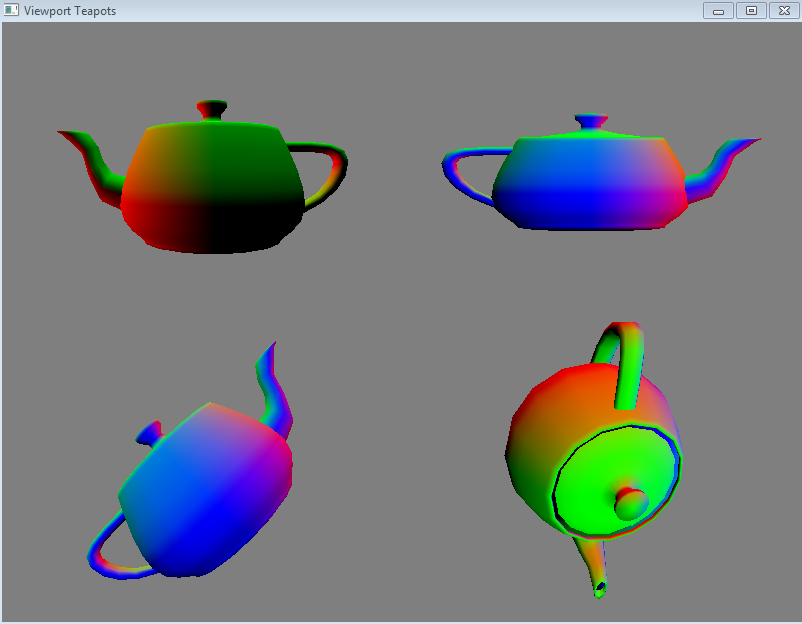
\includegraphics[height=3in]{lab3.PNG}


\section{Rotation}
For this part of the assignmeant I used the rotation functions provided by mathfunc.cpp
\begin{lstlisting}
		if (i > 359)
		{
			i = 0;
		}
		else
		{
			i+=0.03;
		}
		mat4 model1 = rotate_y_deg(rotate_z_deg(rotate_x_deg(identity_mat4(), 3*i),i),5*i);
\end{lstlisting}

\section{Static}
For this part of the assignmeant I didnt really have to do anything as the default position of the teapots was non-spinning.


\section{Two different Perspectives}
For this part of the assignmeant I changed the variables in oone of the perspective functions to achieve a different overall perspective
\begin{lstlisting}
mat4 persp_proj = perspective(45.0, (float)width / (float)height, 0.1, 100.0);
	mat4 persp_proj1 = perspective(90.0, (float)width / (float)height, 0.1, 100.0);
\end{lstlisting}



\section{Orthographic Projection}
For this part of the assignment I wrote an orthographic function in mathfunc.cpp based on the matrix given in the slides. The function simply implements that matrix and multiplies it depending on the inputs given.

\begin{lstlisting}
mat4 Ort = orthograp(-20,20,-20,20,20,-20);
mat4 orthograp(float left, float right, float near, float far,  float top, float bottom ) {	
	mat4 m = zero_mat4(); // make sure bottom-right corner is zero
	m.m[0] = 2/(right-left);
	m.m[5] = 2/(top-bottom);
	m.m[10] = -2/(far-near);
	m.m[3] = -(right + left) /(right-left);
	m.m[7] = -(top + bottom) / (top - bottom);
	m.m[11] = -(far + near)/ (far - near);
	m.m[15] = 1.0f;
	return m;
}
\end{lstlisting}


\section{Look At Function}
Look at Function is implemented using the camera position the teapot piosition and the direction in which 
\begin{lstlisting}
vec3 cam_pos = { 0.0, 0.0, -40.0 };
vec3 teapot_pos = { 0.0,0.0,0.0 };
vec3 up = {0.0,1.0,0.0};
mat4 La = look_at(cam_pos, teapot_pos, up);


\end{lstlisting}
\pagebreak

	
\end{document}